\chapter{GitHub Pages --- Webサイトを無料で公開する}

\section{この章で学ぶこと}

この章では、GitHubリポジトリから直接Webサイトを公開できる\textbf{GitHub Pages}について学びます。具体的には、以下の内容を扱います。

\begin{itemize}
  \item 静的サイトホスティングとは何か、GitHub Pagesはどのような仕組みで動いているのか
  \item ユーザーサイト、プロジェクトサイト、カスタムドメインの3種類の公開URLの違い
  \item ブランチベース、GitHub Actionsベース、ユーザーサイトの3つのセットアップ方法
  \item Jekyllテーマを使ったサイトの見た目のカスタマイズ
  \item 独自ドメイン（カスタムドメイン）の設定方法とHTTPS対応
\end{itemize}

ポートフォリオサイト、プロジェクトのドキュメント、ブログ、技術メモなど、GitHub Pagesは「ちょっとしたWebサイトを手軽に公開したい」という場面で非常に便利なサービスです。サーバーの契約や管理が不要で、GitHubにコードをプッシュするだけでサイトが公開されます。

\section{GitHub Pagesとは}

\subsection{静的サイトホスティングの概念}

Webサイトには大きく分けて\textbf{動的サイト}と\textbf{静的サイト}があります。動的サイトとは、ユーザーのリクエストに応じてサーバー側でHTMLを生成するサイトです。ECサイトの商品検索結果ページやSNSのタイムラインなどが典型例です。動的サイトにはサーバーサイドのプログラム（PHP、Python、Node.jsなど）とデータベースが必要です。

一方、\textbf{静的サイト}は、あらかじめ用意されたHTML、CSS、JavaScriptファイルをそのままブラウザに配信するサイトです。内容が「静的」つまり固定であるため、サーバー側での処理が最小限で済みます。個人のポートフォリオ、プロジェクトのドキュメント、ブログなどは静的サイトとして十分に実現できます。

GitHub Pagesは、この\textbf{静的サイトのホスティング（公開）サービス}です。リポジトリに置いたHTML/CSS/JSファイルを、GitHubのサーバーが自動的にWebサイトとして配信してくれます。レンタルサーバーを契約する必要も、AWSやGCPのようなクラウドサービスの設定を行う必要もありません。

GitHub Pagesの特徴をまとめると、以下のとおりです。

\begin{itemize}
  \item \textbf{完全無料} --- パブリックリポジトリであれば無料で利用できる（プライベートリポジトリでも有料プランで利用可能）
  \item \textbf{HTTPS対応} --- SSL証明書が自動的に発行され、セキュアな通信が標準で有効
  \item \textbf{Gitベースの更新} --- コードをプッシュするだけでサイトが自動更新される
  \item \textbf{Jekyll統合} --- Markdownファイルから自動的にHTMLサイトを生成できる
  \item \textbf{カスタムドメイン対応} --- 独自のドメイン名でサイトを公開できる
\end{itemize}

ただし、静的サイトのホスティングに限定されるため、データベースを使った動的な処理やサーバーサイドのスクリプト実行はできません。また、サイトのサイズには制限があり（推奨1GB以下）、帯域幅にも月間100GBのソフトリミットが設けられています。

\section{公開URLの形式}

GitHub Pagesで公開されるWebサイトのURLは、サイトの種類によって3つの形式があります。それぞれの特徴と使い分けを理解しておきましょう。

\subsection{ユーザーサイト（User Site）}

GitHubアカウントごとに1つだけ作成できる特別なサイトです。\cmd{username.github.io} というリポジトリ名でリポジトリを作成すると、自動的にそのリポジトリの内容が \cmd{https://username.github.io} というURLで公開されます。

ユーザーサイトは、自分自身の紹介ページやポートフォリオとして使われることが多いです。ルートURL（\cmd{/} で始まる）でアクセスできるため、最も短くて覚えやすいURLになります。

\subsection{プロジェクトサイト（Project Site）}

個々のリポジトリごとに作成できるサイトです。リポジトリの Settings → Pages から有効化すると、\cmd{https://username.github.io/repository-name} というURLで公開されます。

たとえば、\cmd{my-library} というリポジトリでGitHub Pagesを有効化すると、\cmd{https://username.github.io/my-library} でアクセスできます。ライブラリやツールのドキュメントサイトとして広く使われています。プロジェクトサイトは数の制限がなく、リポジトリごとに1つずつ作成できます。

\subsection{カスタムドメイン}

\cmd{https://username.github.io} の代わりに、自分で取得した独自ドメイン（例: \cmd{https://example.com}）でサイトを公開することもできます。ドメインレジストラ（お名前.com、Google Domains、Cloudflareなど）でドメインを取得し、DNSレコードを設定する必要があります。設定方法は後述の13.6節で詳しく解説します。

\begin{tabular}{|l|l|l|}
\hline
\textbf{サイトの種類} & \textbf{URL形式} & \textbf{リポジトリ名の条件} \\
\hline
ユーザーサイト & \cmd{https://username.github.io} & \cmd{username.github.io}（固定） \\
\hline
プロジェクトサイト & \cmd{https://username.github.io/repo-name} & 任意 \\
\hline
カスタムドメイン & \cmd{https://your-domain.com} & 任意 \\
\hline
\end{tabular}

\section{セットアップ方法}

GitHub Pagesのセットアップには3つの方法があります。プロジェクトの規模や要件に応じて使い分けましょう。

\subsection{方法1: ブランチから公開（最もシンプル）}

リポジトリの特定のブランチ・ディレクトリをそのままWebサイトとして公開する方法です。最も手軽で、設定ファイルをほとんど書く必要がありません。

\begin{enumerate}
  \item リポジトリの「\textbf{Settings}」タブを開く
  \item 左サイドバーの「\textbf{Pages}」をクリック
  \item 「Build and deployment」セクションで、Sourceを「\textbf{Deploy from a branch}」に設定
  \item \textbf{Branch} でブランチを選択（通常は \cmd{main}）。公開するフォルダは \cmd{/}（ルート）または \cmd{/docs} を選択
  \item 「\textbf{Save}」をクリック
\end{enumerate}

\begin{figure}[htbp]
\centering
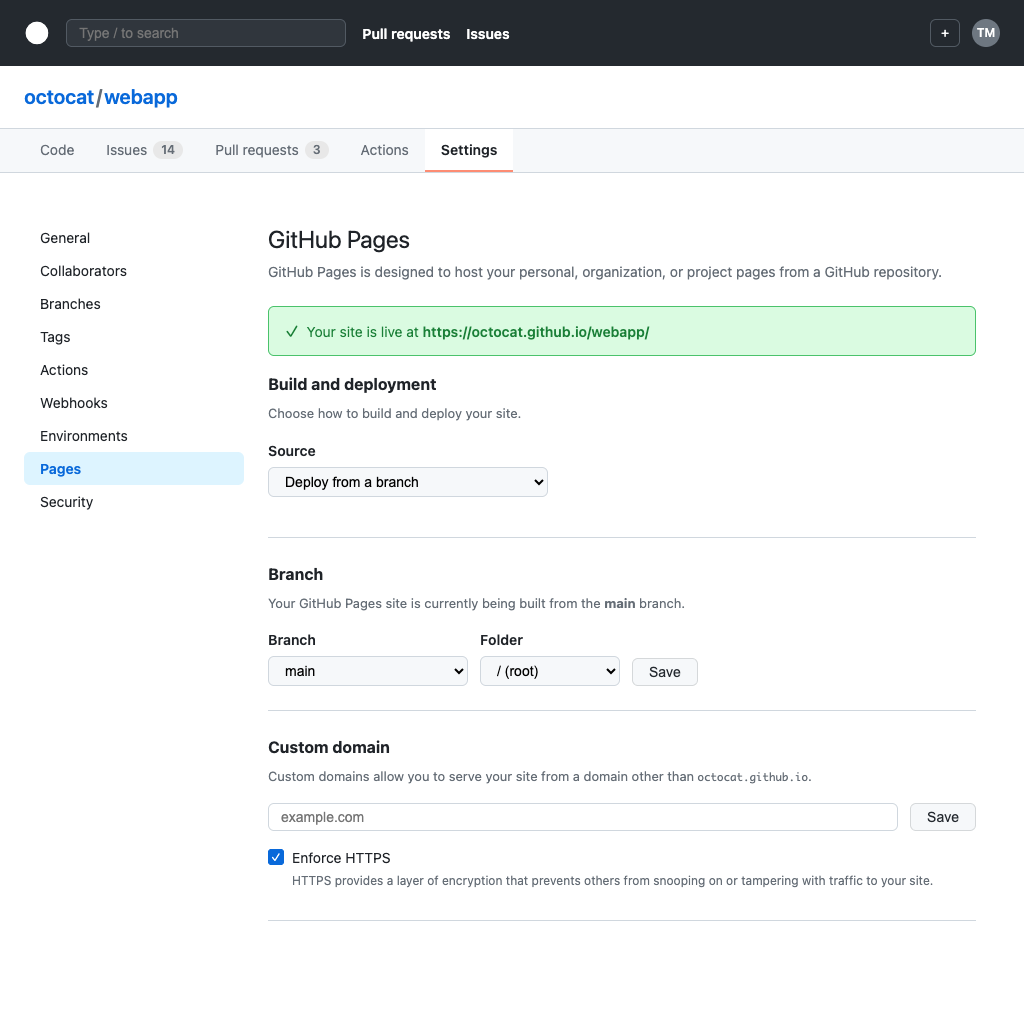
\includegraphics[width=0.95\textwidth]{images/pages-settings.png}
\caption{GitHub Pages設定画面。SourceドロップダウンでDeploy from a branchが選択されている状態}
\end{figure}

数分後には、\cmd{https://username.github.io/repo-name} でサイトにアクセスできるようになります。リポジトリのルートに \cmd{index.html} が存在すれば、それがトップページとして表示されます。\cmd{/docs} フォルダを選択した場合は、\cmd{docs/index.html} がトップページになります。

\cmd{/docs} フォルダの指定は、ソースコードとドキュメントを同じリポジトリで管理したい場合に便利です。ソースコードはリポジトリのルートに、ドキュメント（Webサイト）は \cmd{/docs} ディレクトリに置くことで、両者を明確に分離できます。

\subsection{方法2: GitHub Actionsから公開（柔軟な方法）}

静的サイトジェネレーター（Hugo、Astro、Next.jsなど）を使ってビルドしたサイトを公開する場合や、デプロイ前に何らかの処理を行いたい場合は、GitHub Actionsを使ったデプロイが適しています。

まず、Settings → Pages で Source を「\textbf{GitHub Actions}」に変更します。次に、以下のようなワークフローファイルを作成します。

\begin{lstlisting}[language={}]
# .github/workflows/deploy-pages.yml
name: Deploy to GitHub Pages

on:
  push:
    branches: [main]

permissions:
  contents: read
  pages: write
  id-token: write

concurrency:
  group: "pages"
  cancel-in-progress: false

jobs:
  deploy:
    runs-on: ubuntu-latest
    environment:
      name: github-pages
      url: ${{ steps.deployment.outputs.page_url }}

    steps:
      - name: Checkout
        uses: actions/checkout@v4

      - name: Setup Pages
        uses: actions/configure-pages@v4

      - name: Upload artifact
        uses: actions/upload-pages-artifact@v3
        with:
          path: './public'    # デプロイしたいフォルダを指定

      - name: Deploy to GitHub Pages
        id: deployment
        uses: actions/deploy-pages@v4
\end{lstlisting}

このワークフローのポイントをいくつか補足します。

\textbf{\cmd{permissions}} --- GitHub Pagesへのデプロイには、\cmd{pages: write} と \cmd{id-token: write} の権限が必要です。これを明示的に記述しないと、デプロイステップで権限エラーが発生します。

\textbf{\cmd{concurrency}} --- 複数のデプロイが同時に走ることを防ぐ設定です。\cmd{cancel-in-progress: false} にすると、先に走っているデプロイが完了するまで次のデプロイは待機します。

\textbf{\cmd{path: './public'}} --- デプロイするフォルダを指定します。静的サイトジェネレーターの出力ディレクトリに合わせて変更してください（Hugo なら \cmd{./public}、Next.js の Static Export なら \cmd{./out} など）。

\subsection{方法3: ユーザーサイトの作成}

自分のGitHubアカウントのポートフォリオサイトを作成する場合は、以下の手順が最も簡単です。

\begin{enumerate}
  \item \cmd{username.github.io} という名前のリポジトリを新規作成します（\cmd{username} は自分のGitHub ユーザー名に置き換えてください）
  \item リポジトリに \cmd{index.html} を配置します
  \item mainブランチにプッシュすると、自動的に \cmd{https://username.github.io} で公開されます
\end{enumerate}

簡単な \cmd{index.html} の例を示します。

\begin{lstlisting}[language={}]
<!DOCTYPE html>
<html lang="ja">
<head>
    <meta charset="UTF-8">
    <meta name="viewport" content="width=device-width, initial-scale=1.0">
    <title>My Portfolio</title>
    <style>
        body {
            font-family: -apple-system, BlinkMacSystemFont, 'Segoe UI', sans-serif;
            max-width: 800px;
            margin: 0 auto;
            padding: 2rem;
            line-height: 1.6;
        }
        h1 { color: #333; }
    </style>
</head>
<body>
    <h1>Welcome!</h1>
    <p>This is my portfolio site, hosted on GitHub Pages.</p>
    <h2>Projects</h2>
    <ul>
        <li><a href="https://github.com/username/project-a">Project A</a></li>
        <li><a href="https://github.com/username/project-b">Project B</a></li>
    </ul>
</body>
</html>
\end{lstlisting}

ユーザーサイトは特別な設定なしに公開されるため、GitHub Pagesの動作を試す最も手軽な方法でもあります。

\section{Jekyllテーマの適用}

\subsection{Jekyllとは}

\textbf{Jekyll}は、Ruby製の静的サイトジェネレーターです。Markdownで書いた文章を、テーマに基づいてHTMLサイトに自動変換してくれます。GitHub PagesにはJekyllが組み込まれているため、Rubyを自分のマシンにインストールしなくても、Markdownファイルをプッシュするだけでサイトが生成されます。

HTMLやCSSを一から書かなくても、プロフェッショナルな見た目のサイトが作れるのがJekyllの魅力です。技術ドキュメントやブログに特に適しています。

\subsection{テーマの設定}

リポジトリのルートに \cmd{\_config.yml} を作成し、使いたいテーマを指定します。

\begin{lstlisting}[language={}]
title: My Project Documentation
description: プロジェクトの公式ドキュメント
theme: minima

# リモートテーマ（GitHub Pagesが標準サポートしていないテーマ）を使う場合
# remote_theme: pages-themes/cayman@v0.2.0
\end{lstlisting}

GitHub Pagesが標準でサポートしているテーマには、\cmd{minima}、\cmd{architect}、\cmd{cayman}、\cmd{dinky}、\cmd{hacker}、\cmd{leap-day}、\cmd{merlot}、\cmd{midnight}、\cmd{minimal}、\cmd{modernist}、\cmd{slate}、\cmd{tactile}、\cmd{time-machine} などがあります。

設定画面からテーマを選ぶこともできます。Settings → Pages → 「Theme Chooser」から、プレビューを見ながらテーマを選択できます。

\begin{figure}[htbp]
\centering
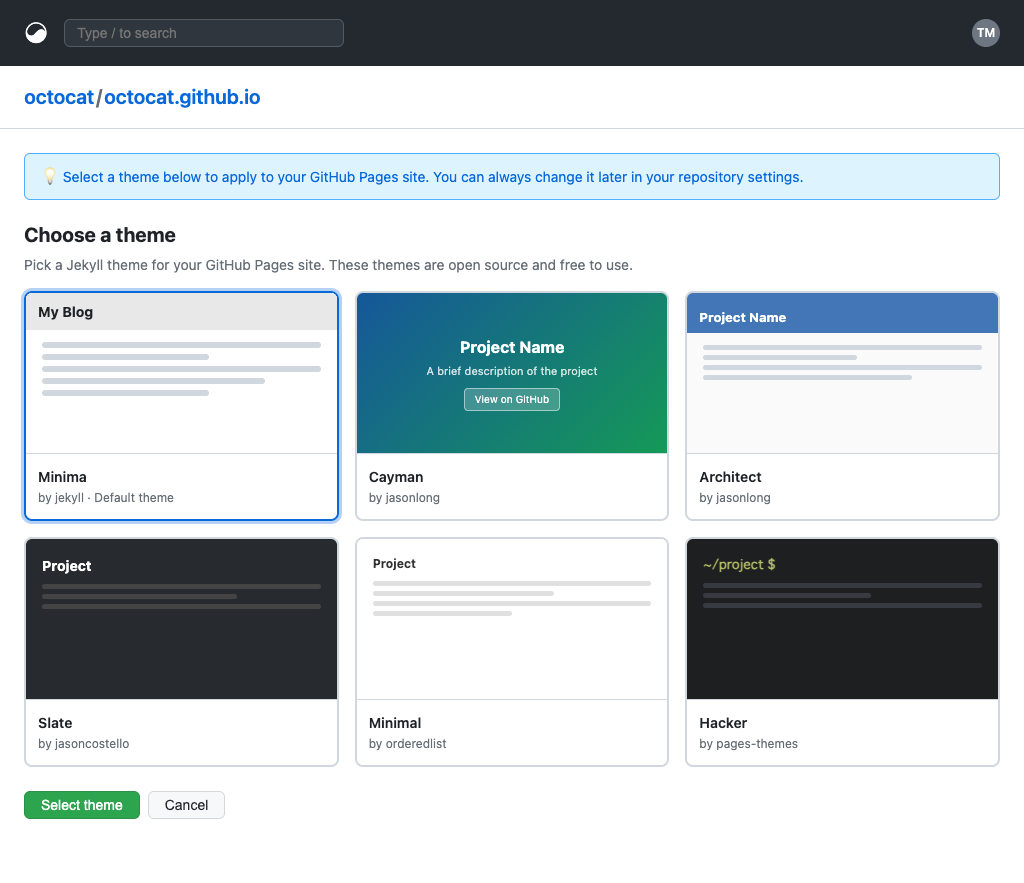
\includegraphics[width=0.95\textwidth]{images/jekyll-themes.png}
\caption{Jekyll テーマ選択画面。複数のテーマのプレビューが表示されている状態}
\end{figure}

\subsection{Markdownでページを作成する}

テーマを設定したら、あとはMarkdownファイルを追加するだけです。ファイルの先頭に\textbf{Front Matter}（YAML形式のメタデータ）を記述することで、Jekyllがそのファイルをページとして認識します。

\begin{lstlisting}[language={}]
---
layout: default
title: About
---

# About This Project

This project provides a simple library for data processing.

## Features

- Fast CSV parsing
- Built-in data validation
- Export to multiple formats
\end{lstlisting}

\cmd{layout: default} は、テーマが提供するデフォルトのレイアウト（ヘッダー、フッター、ナビゲーションなどを含むHTMLの枠組み）を使用することを指示しています。\cmd{title} はページのタイトルで、ブラウザのタブやナビゲーションに表示されます。

リポジトリのルートに置いた \cmd{README.md} も、Jekyllによって自動的にトップページに変換されます。すでに \cmd{README.md} があるリポジトリであれば、テーマを設定するだけでそれなりのサイトが出来上がるのです。

\section{カスタムドメインの設定}

\subsection{なぜカスタムドメインを使うのか}

\cmd{username.github.io} のURLでも十分に機能しますが、プロフェッショナルなプロジェクトや個人ブランディングのためには、独自ドメイン（例: \cmd{docs.myproject.com}）を使いたい場面があります。カスタムドメインを設定すると、GitHub Pagesのサイトに自分のドメインでアクセスできるようになります。

\subsection{DNSレコードの設定}

カスタムドメインを使うには、ドメインのDNSレコードを設定して、そのドメインへのアクセスをGitHub Pagesのサーバーに向ける必要があります。設定方法は、Apex ドメイン（\cmd{example.com}）とサブドメイン（\cmd{www.example.com} や \cmd{docs.example.com}）で異なります。

\textbf{サブドメインの場合（推奨）}

ドメインレジストラのDNS設定画面で、\cmd{CNAME} レコードを追加します。

\begin{tabular}{|l|l|l|}
\hline
\textbf{タイプ} & \textbf{ホスト名} & \textbf{値} \\
\hline
CNAME & \cmd{www} & \cmd{username.github.io} \\
\hline
\end{tabular}

たとえば、\cmd{www.example.com} を使いたい場合は、ホスト名に \cmd{www}、値に \cmd{username.github.io} を設定します。

\textbf{Apexドメインの場合}

Apexドメイン（\cmd{example.com}）を使いたい場合は、\cmd{A} レコードでGitHub PagesのIPアドレスを指定します。

\begin{tabular}{|l|l|l|}
\hline
\textbf{タイプ} & \textbf{ホスト名} & \textbf{値} \\
\hline
A & \cmd{@} & \cmd{185.199.108.153} \\
\hline
A & \cmd{@} & \cmd{185.199.109.153} \\
\hline
A & \cmd{@} & \cmd{185.199.110.153} \\
\hline
A & \cmd{@} & \cmd{185.199.111.153} \\
\hline
\end{tabular}

4つのIPアドレスすべてを登録することで、冗長性が確保されます。

\subsection{GitHub側の設定}

DNSレコードを設定したら、GitHub側でもカスタムドメインを登録します。

\begin{enumerate}
  \item リポジトリの Settings → Pages を開く
  \item 「\textbf{Custom domain}」欄にドメイン名を入力する（例: \cmd{www.example.com}）
  \item 「\textbf{Save}」をクリックする
  \item GitHubがDNSの設定を確認します。正しく設定されていれば、数分以内にチェックマークが表示されます
  \item 「\textbf{Enforce HTTPS}」にチェックを入れる
\end{enumerate}

\begin{figure}[htbp]
\centering
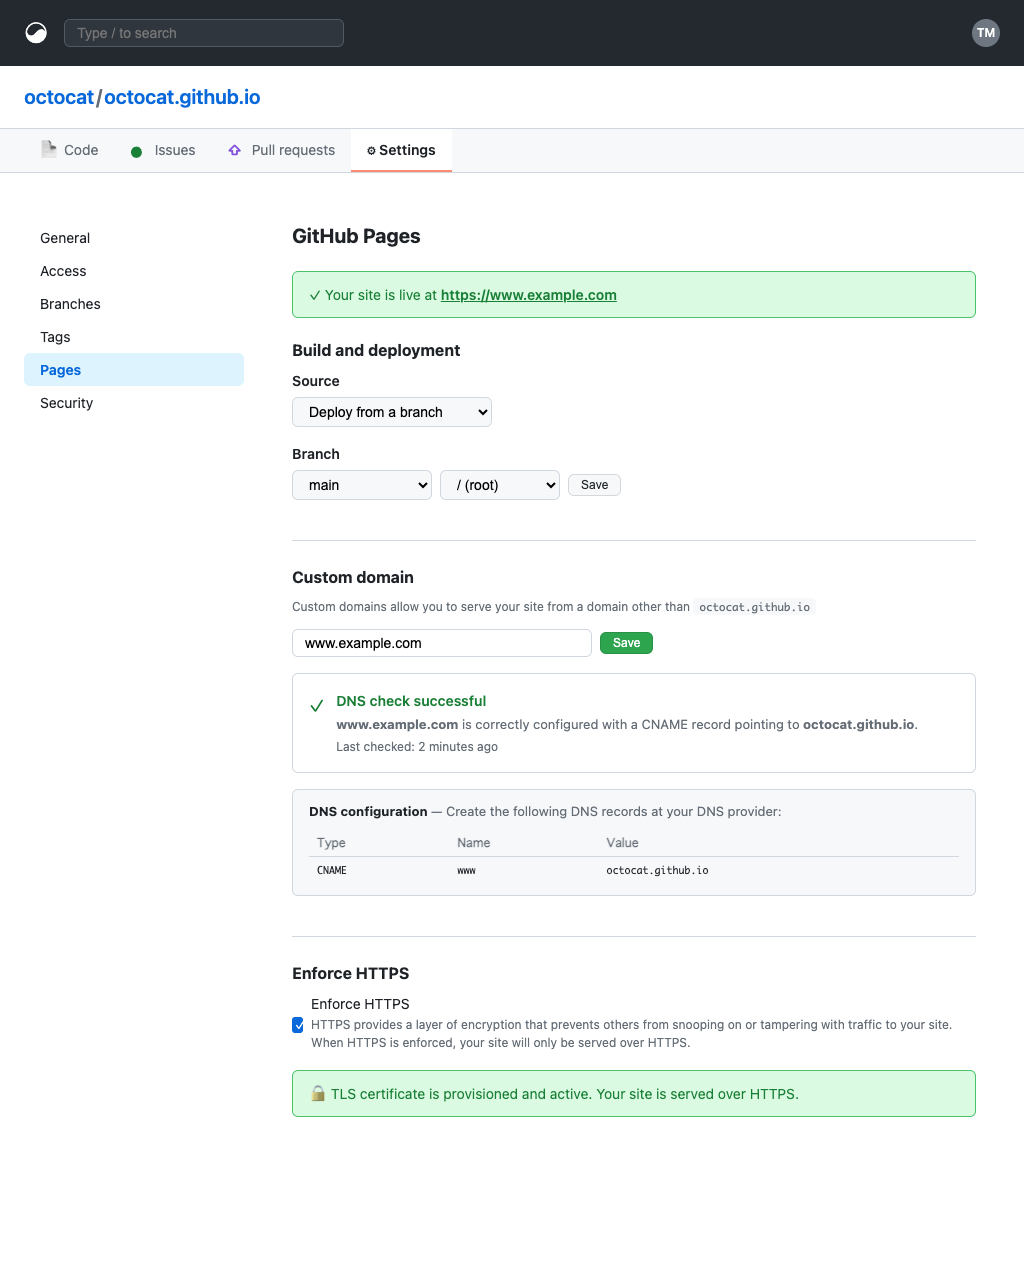
\includegraphics[width=0.95\textwidth]{images/pages-custom-domain.png}
\caption{GitHub PagesのCustom domain設定画面。ドメイン名が入力されDNS checkが成功している状態}
\end{figure}

「Save」をクリックすると、リポジトリのルートに \cmd{CNAME} という名前のファイルが自動的に作成されます。このファイルにはドメイン名が1行だけ書かれています。

\begin{lstlisting}[language={}]
www.example.com
\end{lstlisting}

このファイルは手動で作成しても構いません。重要なのは、このファイルがリポジトリに存在することです。

\subsection{HTTPS対応}

GitHub Pagesでは、カスタムドメインに対しても\textbf{無料でSSL/TLS証明書が自動発行}されます。「Enforce HTTPS」を有効にすると、HTTPでのアクセスが自動的にHTTPSにリダイレクトされます。

DNSの設定が反映されてから証明書が発行されるまでに、最大24時間かかることがあります。「Enforce HTTPS」のチェックボックスがグレーアウトしている場合は、DNS設定の反映を待っている状態です。しばらく待ってからページを再読み込みしてみてください。

\section{まとめ}

この章では、GitHub Pagesを使ったWebサイトの公開方法を学びました。

\begin{itemize}
  \item \textbf{GitHub Pages}は、GitHubリポジトリから直接静的Webサイトをホスティングできる無料サービスです
  \item \textbf{ユーザーサイト}（\cmd{username.github.io}）は1つだけ、\textbf{プロジェクトサイト}（\cmd{username.github.io/repo}）はリポジトリごとに作成できます
  \item セットアップは\textbf{ブランチベース}（最も簡単）、\textbf{GitHub Actionsベース}（柔軟）、\textbf{ユーザーサイト}（特定リポジトリ名）の3つの方法があります
  \item \textbf{Jekyll}テーマを適用すると、Markdownファイルからプロフェッショナルな見た目のサイトが自動生成されます
  \item \textbf{カスタムドメイン}を使う場合は、DNSレコード（CNAMEまたはAレコード）を設定し、GitHub側でドメインを登録します。HTTPSは無料で自動対応されます
\end{itemize}

GitHub Pagesは、「サーバー管理の知識がなくても、コードをプッシュするだけでWebサイトが公開できる」という手軽さが最大の魅力です。プロジェクトのドキュメント公開から個人のポートフォリオまで、幅広い用途に活用できます。
